\documentclass[14pt]{beamer}
%
% Choose how your presentation looks.
%
% For more themes, color themes and font themes, see:
% http://deic.uab.es/~iblanes/beamer_gallery/index_by_theme.html
%
\mode<presentation>
{
  \usetheme{default}      % or try Darmstadt, Madrid, Warsaw, ...
  \usecolortheme{default} % or try albatross, beaver, crane, ...
  \usefonttheme{default}  % or try serif, structurebold, ...
  \setbeamertemplate{navigation symbols}{}
  \setbeamertemplate{caption}[numbered]
} 

\addtobeamertemplate{navigation symbols}{}{%
    \usebeamerfont{footline}%
    \usebeamercolor[fg]{footline}%
    \hspace{1em}%
    \insertframenumber/\inserttotalframenumber
}
\usepackage[english]{babel}
\usepackage{cite}
\usepackage[numbers]{natbib}
% \usepackage[authoryear]{natbib}
\usepackage[utf8x]{inputenc}
\usepackage{xcolor,colortbl}
\definecolor{Gray}{gray}{0.85}
\definecolor{LightCyan}{rgb}{0.88,1,1}
\newcommand{\red}[1]{\textcolor{red}{#1}}

\title[Your Short Title]{Refresh Strategies for Continuous Active Learning}
\author{Nimesh Ghelani\\Supervisor: Mark D. Smucker}
\institute{University of Waterloo}
\date{}

\begin{document}
\setbeamertemplate{caption}{\raggedright\insertcaption\par}

\begin{frame}
  \titlepage
\end{frame}

\section{Introduction}
\begin{frame}{Introduction}
    Find all or nearly all relevant documents using minimal assessment costs
    \vskip 1cm

    \pause
    \textbf{High Recall Problem: } How to achieve high recall with high overall
    precision?
    \vskip 1cm
    Recall $\leftarrow$ fraction of relevant documents retrieved
    Precision $\leftarrow$ fraction of retrieved documents which are relevant
\end{frame}

\begin{frame}{Introduction}
    Real world high-recall problems:

    \begin{itemize}
    \item Systematic review in medicine~\cite{yu2016read}
            \begin{itemize}
                \item Exhaustive literature review to answer a research question
            \end{itemize}
        \pause
        \item Legal eDiscovery~\cite{oard2013information}
        \begin{itemize}
            \item Exchange of evidence between parties in a lawsuit
        \end{itemize}
        \pause
        \item Building test collection
            \begin{itemize}
                \item TREC style evaluation
                \item NIST assessors review documents from a pool created by
                    participating systems~\cite{harman1993overview}
            \end{itemize}
    \end{itemize}

\end{frame}

\begin{frame}{Introduction}
    \begin{itemize}
        \item Legal eDiscovery
        \item Systematic review in medicine
        \item Building test collection
    \end{itemize}
    \vskip 0.5cm
    Common properties:
    \begin{itemize}
        \item Desirable to retrieve (nearly) all relevant documents
        \item Significant increase in the size of the data
        \item Humans are the most expensive part of the process
    \end{itemize}

\end{frame}

\begin{frame}{Introduction}
    Technology Assisted Review (TAR): computer-assisted methods to do eDiscovery

    \vskip 1cm
    \pause
    Continuous Active Learning (CAL)~\cite{cormack2014evaluation}:
    \begin{itemize}
        \item A TAR protocol
        \item Human in loop with a machine learning model
    \end{itemize}
\end{frame}

\begin{frame}{Introduction}
\begin{figure}
 \centering 
 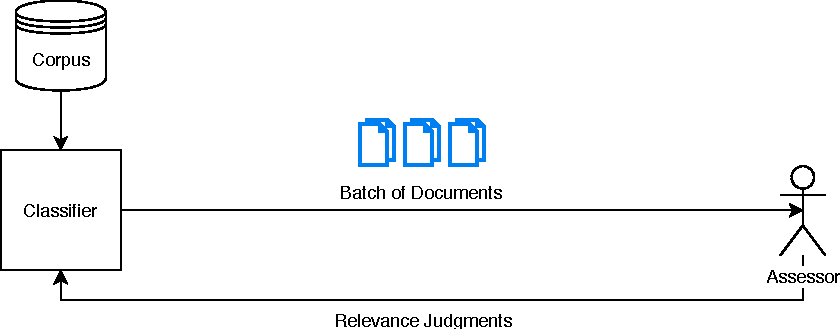
\includegraphics[width=1.0\textwidth]{animation/1.pdf}
 \caption{Relevance Feedback Loop}
\end{figure}
\end{frame}

\begin{frame}{Introduction}
\begin{figure}
 \centering 
 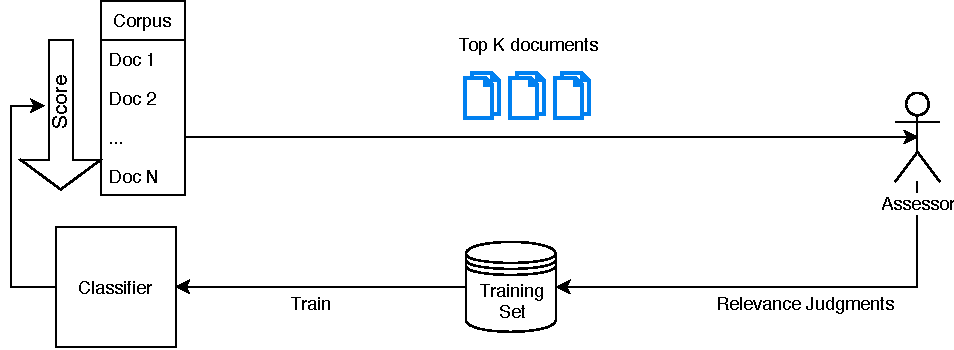
\includegraphics[width=1.0\textwidth]{animation/2.pdf}
 \caption{Relevance Feedback Loop in Continuous Active Learning}
\end{figure}
\end{frame}

\begin{frame}{Introduction}
\begin{figure}
 \centering 
 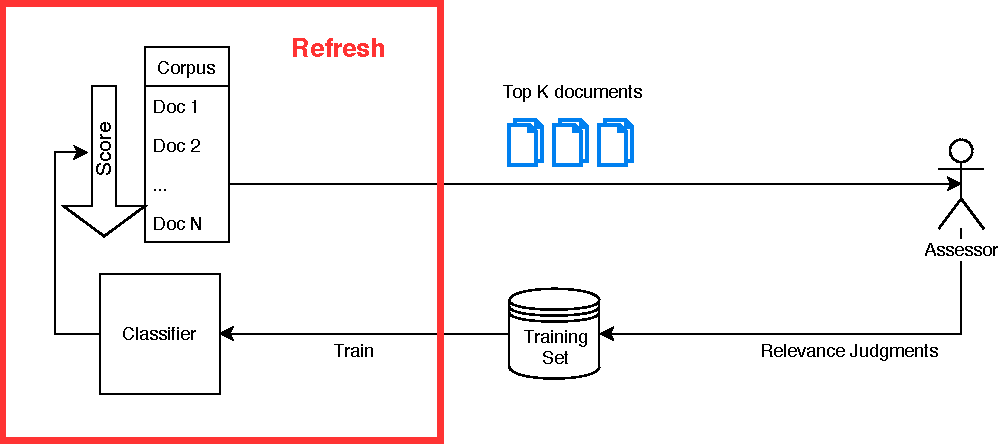
\includegraphics[width=1.0\textwidth]{animation/3.pdf}
 \caption{Relevance Feedback Loop in Continuous Active Learning}
\end{figure}
\end{frame}

\begin{frame}{Introduction}
Refresh:
\begin{itemize}
    \item Use available judgments to build a classifier
    \item Produce next set of documents to be judged
\end{itemize}

\pause
\vskip 0.5cm
Refresh strategy controls
\begin{itemize}
    \item When to refresh?
    \item How to refresh?
\end{itemize}

\pause
\vskip 0.5cm
Refresh strategy doesn't control
\begin{itemize}
    \item Feature engineering
    \item Bootstrapping
    \item User Interface
    \item When to stop?
\end{itemize}
\end{frame}

\begin{frame}{Objectives}
\begin{itemize}
    \item Investigate various refresh strategies
        \begin{itemize}
            \item effectiveness and efficiency
        \end{itemize}
    \item A modern implementation of the CAL framework
        \begin{itemize}
            \item fast and extensible
            \item research and practical use
        \end{itemize}
\end{itemize}
\end{frame}

\begin{frame}{Outline}
\begin{itemize}
    \item Refresh Strategies
    \begin{itemize}
        \item Static batch sizes
        \item Exponential batch sizes
        \item Partial refresh
        \item Precision based
        \item Recency Weighting
        % \item Forgetting
    \end{itemize}
    \item Implementation
    \item Dataset and Experiment
    \item Results
    \item Summary
    \item Future Work
\end{itemize}
\end{frame}

\begin{frame}{Outline}
\begin{itemize}
    \item Refresh Strategies
    \begin{itemize}
        \item \red{Static batch sizes}
        \item Exponential batch sizes
        \item Partial refresh
        \item Precision based
        \item Recency Weighting
        % \item Forgetting
    \end{itemize}
    \item Implementation
    \item Dataset and Experiment
    \item Results
    \item Summary
    \item Future Work
\end{itemize}
\end{frame}

\begin{frame}{Static Batch Strategy}
\begin{figure}
 \centering 
 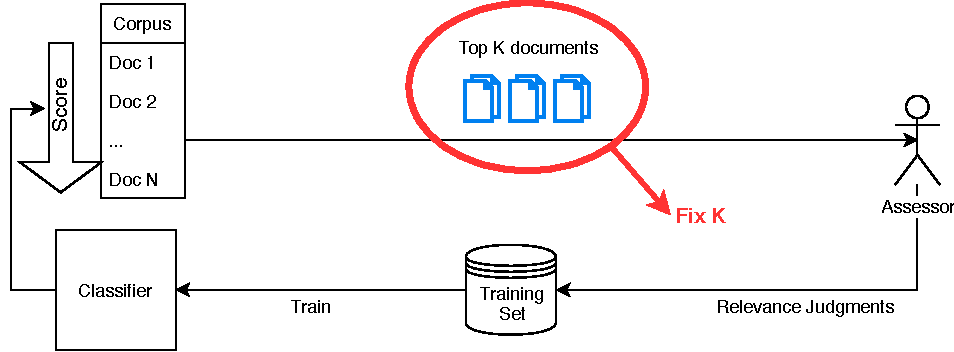
\includegraphics[width=1.0\textwidth]{animation/static.pdf}
 \caption{Static Batch Strategy}
\end{figure}
\end{frame}

\begin{frame}{Static Batch Strategy}
\begin{figure}
 \centering 
 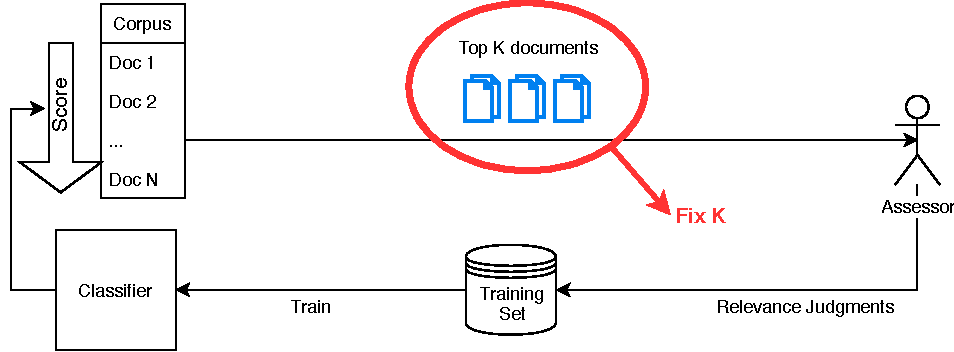
\includegraphics[width=0.8\textwidth]{animation/static.pdf}
\end{figure}
\begin{itemize}
    \item \texttt{k=1000} in earlier version of CAL
    \item \texttt{k=1} $\rightarrow$ maximum refresh frequency
\end{itemize}
\end{frame}


\begin{frame}{Outline}
\begin{itemize}
    \item Refresh Strategies
    \begin{itemize}
        \item Static batch sizes
        \item \red{Exponential batch sizes}
        \item Partial refresh
        \item Precision based
        \item Recency Weighting
        % \item Forgetting
    \end{itemize}
    \item Implementation
    \item Dataset and Experiment
    \item Results
    \item Summary
    \item Future Work
\end{itemize}
\end{frame}

\begin{frame}{Exponential Batch Strategy}
Train and score all documents every $K$ assessments ($K$ increases exponentially)

\vskip 1cm
After every refresh,
$K← K + (K + 9)/10$
\vskip 0.5cm
\pause
For every $E$ documents judged by an assessor, $O(\log E)$ number of refreshes
are performed
\end{frame}

\begin{frame}{Exponential Batch Strategy}
Used in the Baseline Model Implementation (BMI) at the TREC 2015 and 2016 Total
Recall tracks~\cite{roegiest2015trec,grossman2016trec}

\vskip 1cm
None of the participating teams were able to outperform the baseline

\end{frame}

\begin{frame}{Outline}
\begin{itemize}
    \item Refresh Strategies
    \begin{itemize}
        \item Static batch sizes
        \item Exponential batch sizes
        \item \red{Partial refresh}
        \item Precision based
        \item Recency Weighting
        % \item Forgetting
    \end{itemize}
    \item Implementation
    \item Dataset and Experiment
    \item Results
    \item Summary
    \item Future Work
\end{itemize}
\end{frame}

\subsection{Partial Refresh}
\begin{frame}{Partial Refresh Strategy}
    \textbf{Motivation:} Avoid scoring the entire corpus every time
\vskip 0.5cm
\textbf{Observation:} Classifier's notion of relevance doesn't change drastically between
subsequent judgments

\end{frame}

\begin{frame}{Partial Refresh Strategy}
\begin{figure}
 \centering 
 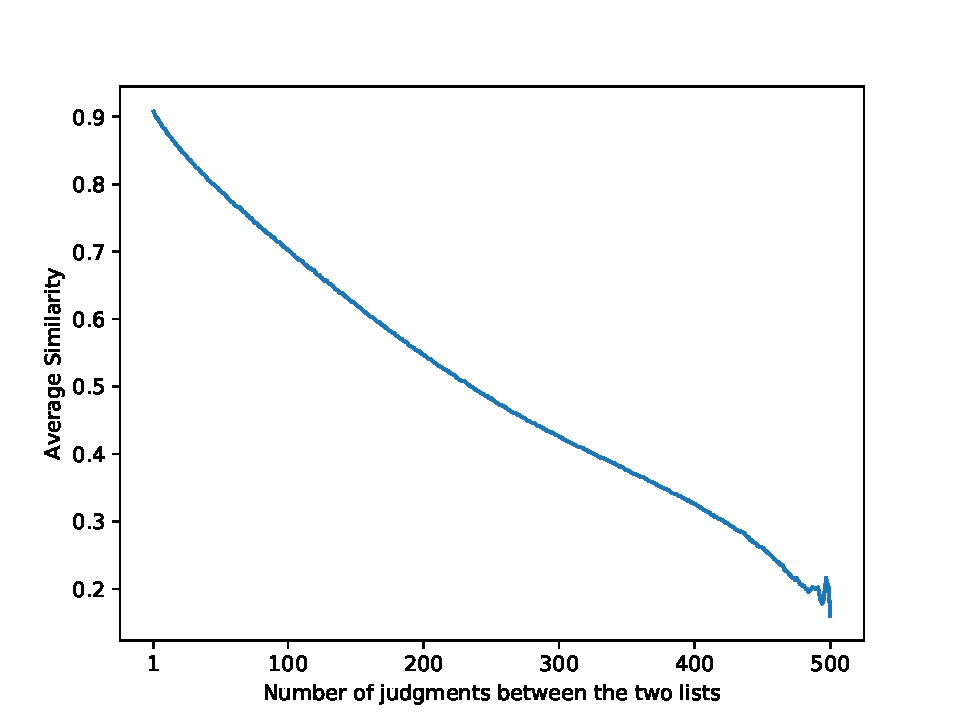
\includegraphics[width=0.7\textwidth]{../plots/ranklist_similarity.pdf}
 \caption{Average set similarity between two ranked lists (truncated at 1000)
 separated by various number of judgments; when refreshing after every judgment}
\end{figure}
\end{frame}

\begin{frame}{Partial Refresh Strategy}
\textbf{Definition:}

\vskip 0.7cm
Perform frequent scoring on a smaller set of data
\vskip 0.4cm
Periodic complete scoring
\end{frame}


\begin{frame}{Partial Refresh Strategy}
\begin{figure}
 \centering 
 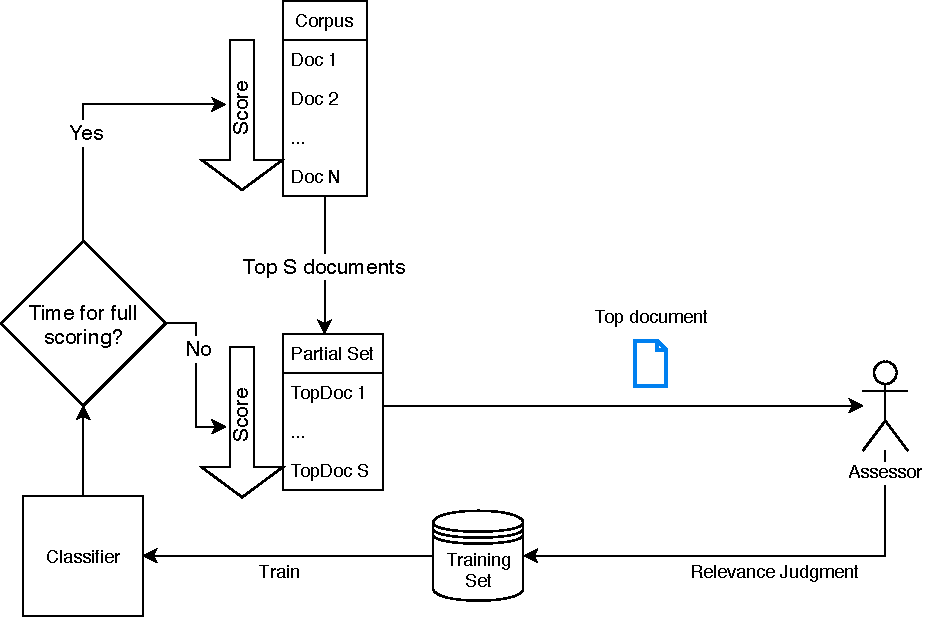
\includegraphics[width=1.0\textwidth]{animation/partial.pdf}
 \caption{Partial Refresh Strategy}
\end{figure}
\end{frame}

\begin{frame}{Partial Refresh Strategy}
\begin{figure}
 \centering 
 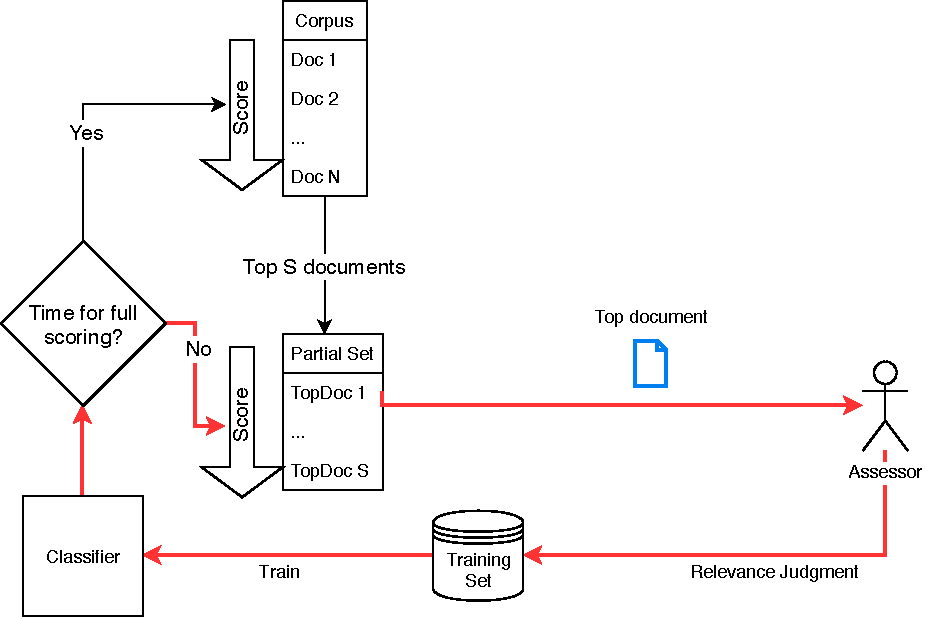
\includegraphics[width=1.0\textwidth]{animation/partial1.pdf}
 \caption{After every judgment}
\end{figure}
\end{frame}

\begin{frame}{Partial Refresh Strategy}
\begin{figure}
 \centering 
 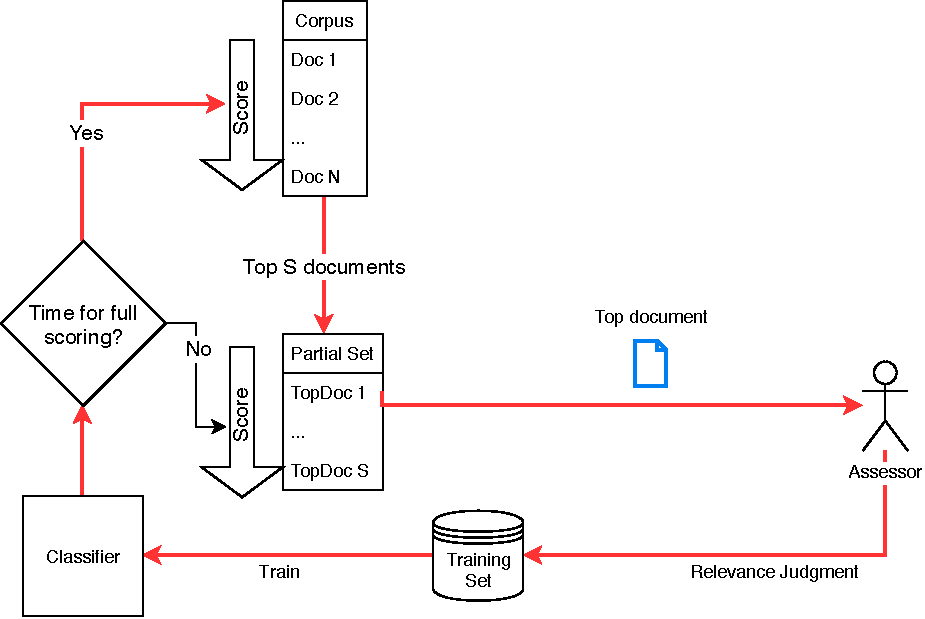
\includegraphics[width=1.0\textwidth]{animation/partial2.pdf}
 \caption{After every K judgments}
\end{figure}
\end{frame}

\begin{frame}{Partial Refresh Strategy}
    Two parameters:
    \begin{itemize}
        \item $K \rightarrow$ Frequency of full scoring
        \item $S \rightarrow$ Size of the partial set
    \end{itemize}
\end{frame}

\begin{frame}{Partial Refresh Strategy}
    When working with a large corpus:
    \begin{itemize}
        \item Not enough memory to load all the document features
        \item Scoring with disk access very slow
    \end{itemize}
    \pause
    \vskip 0.5cm
    Modified partial refresh strategy:
    \begin{itemize}
        \item Store the smaller partial set in memory
        \item Perform full scoring with disk reads in the background
    \end{itemize}
\end{frame}


\begin{frame}{Outline}
\begin{itemize}
    \item Refresh Strategies
    \begin{itemize}
        \item Static batch sizes
        \item Exponential batch sizes
        \item Partial refresh
        \item \red{Precision based}
        \item Recency Weighting
        % \item Forgetting
    \end{itemize}
    \item Implementation
    \item Dataset and Experiment
    \item Results
    \item Summary
    \item Future Work
\end{itemize}
\end{frame}

\begin{frame}{Precision Based Refreshing}
    \textbf{Motivation:} Investigate factors more meaningful than ``elapsed number
    of judgments''
    \pause
\vskip 1cm
\textbf{Definition:} Refresh when ``output quality'' falls below some threshold
\vskip 0.5cm
\textbf{Problem:} Defining ``output quality''

\pause
\vskip 1cm
Refresh when the precision of the last $m$ assessed documents fall below $p$
\end{frame}

% \begin{frame}{Precision Based Refreshing}
% \begin{figure}
%  \centering 
%  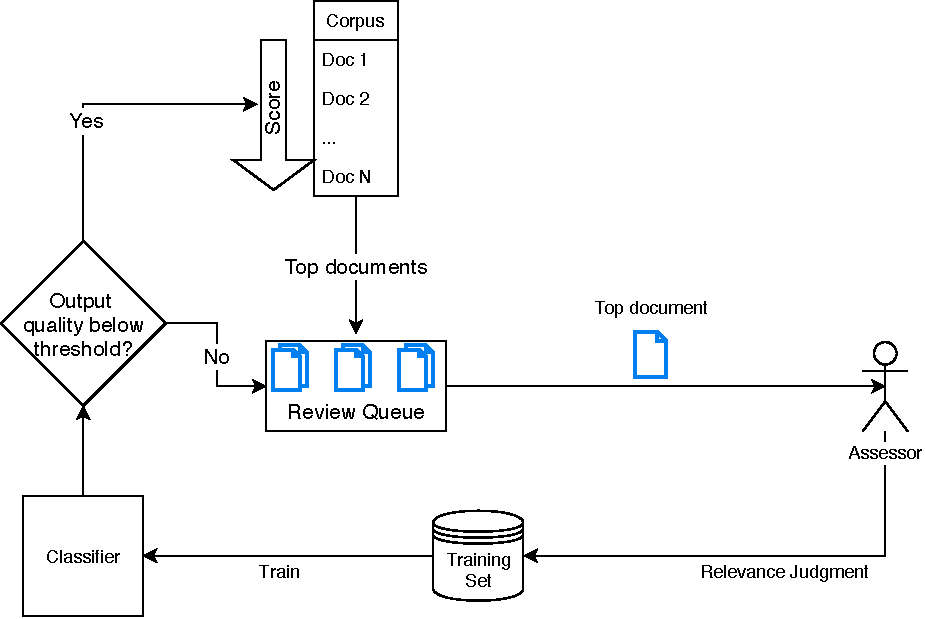
\includegraphics[width=1.0\textwidth]{animation/prec.pdf}
% \end{figure}
% \end{frame}


\begin{frame}{Outline}
\begin{itemize}
    \item Refresh Strategies
    \begin{itemize}
        \item Static batch sizes
        \item Exponential batch sizes
        \item Partial refresh
        \item Precision based
        \item \red{Recency Weighting}
        % \item Forgetting
    \end{itemize}
    \item Implementation
    \item Dataset and Experiment
    \item Results
    \item Summary
    \item Future Work
\end{itemize}
\end{frame}

\begin{frame}{Recency Weighting Strategy}
Recent judgments prioritized during training
\vskip 1cm

\textbf{Original Motivation:} Improve the quality of the logistic regression classifier
\pause
\centerline{\textit{It didn't!}}
\pause
\vskip 1cm

\textbf{Motivation:} Improve quality of a weakened but faster training algorithm
\end{frame}


\begin{frame}{Recency Weighting Strategy}
    Training algorithm used in CAL: pegasos learner with ROC
    sampling~\cite{sculley2010combined}

\begin{itemize}
    \item Several number of iterations
    \item In each iteration:
        \begin{itemize}
            \item randomly sample a positive and a negative document
            \item compute loss on their difference
            \item update weights
        \end{itemize}
\end{itemize}

\pause
Weaken the training by reducing the number of iterations
\end{frame}

\begin{frame}{Recency Weighting Strategy}
Recent judgments prioritized during training
\vskip 1cm

\textbf{Default training:} Uniform random sampling of document

\pause
\vskip 0.5cm
\textbf{Modified training:} latest judged document is $w$ times more likely to be
sampled than the first judgment (fit a linear curve).
\end{frame}


\begin{frame}{Outline}
\begin{itemize}
    \item Refresh Strategies
    \begin{itemize}
        \item Static batch sizes
        \item Exponential batch sizes
        \item Partial refresh
        \item Precision based
        \item Recency Weighting
        % \item Forgetting
    \end{itemize}
    \item \red{Implementation}
    \item Dataset and Experiment
    \item Results
    \item Summary
    \item Future Work
\end{itemize}
\end{frame}

\begin{frame}{Implementation}
    Modern C++ implementation of a generalized CAL framework
    \begin{itemize}
        \item Initially developed as part of
            HiCAL~\footnote{\url{https://hical.github.io}}, an open source tool
            we build for TREC 2017 Core Track~\cite{zhang2017uwaterloomds,
            sigirdemo}
        \item Designed for efficiency
        \item Extensible
            \begin{itemize}
                \item implement new refresh strategies
            \end{itemize}
        \item Easy to use in practical applications
            \begin{itemize}
                \item Command line tool for running simulations
                \item HTTP API
            \end{itemize}
    \end{itemize}
\end{frame}


\begin{frame}{Outline}
\begin{itemize}
    \item Refresh Strategies
    \begin{itemize}
        \item Static batch sizes
        \item Exponential batch sizes
        \item Partial refresh
        \item Precision based
        \item Recency Weighting
        % \item Forgetting
    \end{itemize}
    \item Implementation
    \item \red{Dataset and Experiment}
    \item Results
    \item Summary
    \item Future Work
\end{itemize}
\end{frame}

\begin{frame}{Dataset and Experiment}
    \begin{itemize}
        \item \texttt{Athome1} test collection from the TREC 2015 Total Recall
            track~\cite{roegiest2015trec}
        \item Around 290k documents (emails); 10 topics
        \item Implementation of CAL from HiCAL
            \begin{itemize}
                \item Scoring on single thread
            \end{itemize}
        \item 4398 avg. number of relevant documents per topic
    \end{itemize}
\end{frame}

\begin{frame}{Evaluation}
    \begin{itemize}
        \item Recall = $\frac{\text{No. of relevant documents retrieved}}{\text{Total no. of
        relevant documents}}$
        \item Effort = No. of documents judged by the assessor
        \item Normalized Effort = $\frac{\text{No. of
                    Assessments}}{\text{Total no. of
            relevant documents}}$
    \end{itemize}
\end{frame}

\begin{frame}{Evaluation}
    \begin{itemize}
        \item Gain curve
            \begin{itemize}
                \item Plot of recall against normalized effort
            \end{itemize}
        \pause
        \item Recall at certain values of normalized effort (1, 1.5, 2)
        \item Effort required to achieve 75\% recall
        \pause
        \item Simulation running time (stopping criteria: $E_{norm} = 2$)
            \begin{itemize}
                \item Scoring time
                \item Training time
            \end{itemize}
    \end{itemize}
\end{frame}


\begin{frame}{Outline}
\begin{itemize}
    \item Refresh Strategies
    \begin{itemize}
        \item Static batch sizes
        \item Exponential batch sizes
        \item Partial refresh
        \item Precision based
        \item Recency Weighting
        % \item Forgetting
    \end{itemize}
    \item Implementation
    \item Dataset and Experiment
    \item \red{Results}
    \item Summary
    \item Future Work
\end{itemize}
\end{frame}

\begin{frame}{Results}
\begin{table}[]
\centering
\caption{Exponential vs Static Batch}
\label{table.summary}
\resizebox{\textwidth}{!}{%
\begin{tabular}{|c|c|c|c|c|c|}
\hline
\textbf{Strategy} & \begin{tabular}[x]{@{}c@{}}
    \textbf{Avg. Recall}\\ \textbf{@($E_{norm}$=1)}
\end{tabular} & \begin{tabular}[x]{@{}c@{}}
\textbf{Avg. Recall}\\ \textbf{@($E_{norm}$=2)}
\end{tabular} & \begin{tabular}[x]{@{}c@{}}
\textbf{$E_{norm}$ for}\\ \textbf{75\% recall}
\end{tabular}&
\begin{tabular}[x]{@{}c@{}}
    \textbf{Running Time}\\ \textbf{(in min)}
\end{tabular} \\ \hline \hline
\texttt{exponential}& 0.715 & 0.905 & 1.128 & 0.3 \\ \hline \hline
\rowcolor{LightCyan}
\texttt{static(k=1)} & 0.750 & 0.926 & 1.021 & 59.59 \\ \hline
\texttt{static(k=100)} &  0.704 & 0.887 & 1.167 & 0.59 \\ \hline
\end{tabular}
}
\end{table}
\vskip 0.5cm
\texttt{exponential}: exponentially increasing batch size
\texttt{static(k)}: fixed batch size of \texttt{k}
\end{frame}

\begin{frame}{Results}
\begin{figure}
 \centering 
 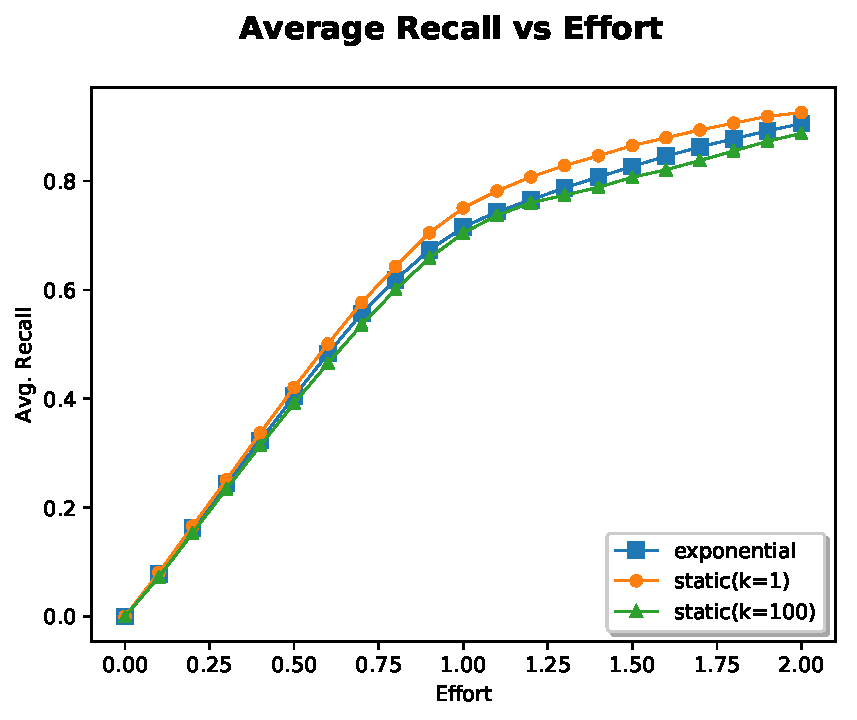
\includegraphics[width=0.7\textwidth]{../plots/bmi_static.pdf}
 \caption{Exponential vs Static Batch}
\end{figure}
\end{frame}

\begin{frame}{Results}
\begin{table}[]
\centering
\caption{Partial Refresh Strategy}
\label{table.summary}
\resizebox{\textwidth}{!}{%
\begin{tabular}{|c|c|c|c|c|c|}
\hline
\textbf{Strategy} & \begin{tabular}[x]{@{}c@{}}
    \textbf{Avg. Recall}\\ \textbf{@($E_{norm}$=1)}
\end{tabular} & \begin{tabular}[x]{@{}c@{}}
\textbf{Avg. Recall}\\ \textbf{@($E_{norm}$=2)}
\end{tabular} & \begin{tabular}[x]{@{}c@{}}
\textbf{$E_{norm}$ for}\\ \textbf{75\% recall}
\end{tabular}&
\begin{tabular}[x]{@{}c@{}}
    \textbf{Running Time}\\ \textbf{(in min)}
\end{tabular} \\ \hline \hline
\rowcolor{LightCyan}
\texttt{static(k=1)} & 0.750 & 0.926 & 1.021 & 59.59 \\ \hline \hline
\texttt{partial(k=10,s=1000)} &  0.753 & 0.926 & 1.008 & 38.72 \\ \hline
\rowcolor{LightCyan}
% \texttt{partial(k=100,s=500)} &  0.753 & 0.923 & 1.022 & 38.28 \\ \hline
% \rowcolor{LightCyan}
\texttt{partial(k=100,s=1000)} &  0.754 & 0.922 & 1.013 & 36.52 \\ \hline
\rowcolor{LightCyan}
\texttt{partial(k=100,s=5000)} &  0.756 & 0.921 & 1.016 & 47.19 \\ \hline
\texttt{partial(k=500,s=1000)} &  0.700 & 0.815 & 1.324 & 35.77 \\
\hline
\end{tabular}
}
\end{table}
\vskip 0.5cm
\texttt{static(k)}: fixed batch size of \texttt{k}

\texttt{partial(k,s)}: complete scoring after \texttt{k} judgments, partial set
size of \texttt{s} documents
\end{frame}

\begin{frame}{Results}
\begin{table}[]
\centering
\caption{Partial Refresh Strategy}
\label{table.summary}
\resizebox{\textwidth}{!}{%
\begin{tabular}{|c|c|c|c|c|c|}
\hline
\textbf{Strategy} & \begin{tabular}[x]{@{}c@{}}
    \textbf{Avg. Recall}\\ \textbf{@($E_{norm}$=1)}
\end{tabular} & \begin{tabular}[x]{@{}c@{}}
\textbf{Avg. Recall}\\ \textbf{@($E_{norm}$=2)}
\end{tabular} & \begin{tabular}[x]{@{}c@{}}
\textbf{$E_{norm}$ for}\\ \textbf{75\% recall}
\end{tabular}&
\begin{tabular}[x]{@{}c@{}}
    \textbf{Scoring Time}\\ \textbf{(in min)}
\end{tabular} \\ \hline \hline
\rowcolor{LightCyan}
\texttt{static(k=1)} & 0.750 & 0.926 & 1.021 & 22.89 \\ \hline \hline
\texttt{partial(k=10,s=1000)} &  0.753 & 0.926 & 1.008 & 2.46 \\ \hline
% \rowcolor{LightCyan}
% \texttt{partial(k=100,s=500)} &  0.753 & 0.923 & 1.022 & 38.28 \\ \hline
\rowcolor{LightCyan}
\texttt{partial(k=100,s=1000)} &  0.754 & 0.922 & 1.013 & 0.38 \\ \hline
\rowcolor{LightCyan}
\texttt{partial(k=100,s=5000)} &  0.756 & 0.921 & 1.016 & 1.00 \\ \hline
\texttt{partial(k=500,s=1000)} &  0.700 & 0.815 & 1.324 & 0.17 \\
\hline
\end{tabular}
}
\end{table}
\vskip 0.5cm
\texttt{static(k)}: fixed batch size of \texttt{k}

\texttt{partial(k,s)}: complete scoring after \texttt{k} judgments, partial set
size of \texttt{s} documents
\end{frame}

\begin{frame}{Results}
\begin{figure}
 \centering 
 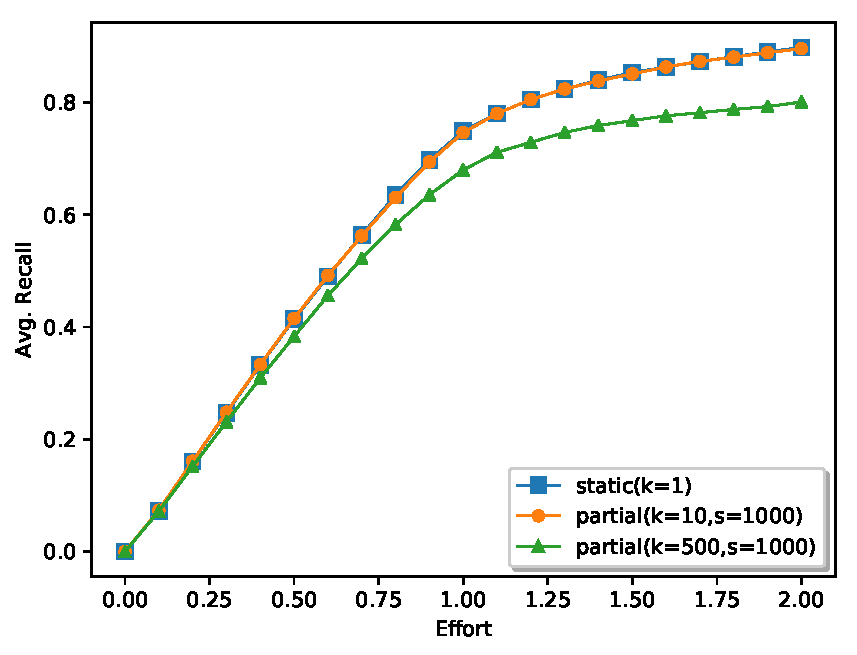
\includegraphics[width=0.7\textwidth]{../plots/static_partial.pdf}
 \caption{Partial vs Static Batch}
\end{figure}
\end{frame}

\begin{frame}{Results}
\begin{table}[]
\centering
\caption{Precision Based Refreshing}
\label{table.summary}
\resizebox{\textwidth}{!}{%
\begin{tabular}{|c|c|c|c|c|c|}
\hline
\textbf{Strategy} & \begin{tabular}[x]{@{}c@{}}
    \textbf{Avg. Recall}\\ \textbf{@($E_{norm}$=1)}
\end{tabular} & \begin{tabular}[x]{@{}c@{}}
\textbf{Avg. Recall}\\ \textbf{@($E_{norm}$=2)}
\end{tabular} & \begin{tabular}[x]{@{}c@{}}
\textbf{$E_{norm}$ for}\\ \textbf{75\% recall}
\end{tabular}&
\begin{tabular}[x]{@{}c@{}}
    \textbf{Running Time}\\ \textbf{(in min)}
\end{tabular} \\ \hline \hline
\rowcolor{LightCyan}
\texttt{static(k=1)} & 0.750 & 0.926 & 1.021 & 59.59 \\ \hline \hline
\texttt{precision(m=25,p=0.4)} &  0.698 & 0.915 & 1.129 & 35.16 \\ \hline
\texttt{precision(m=25,p=0.6)} &  0.735 & 0.923 & 1.059 & 39.44 \\ \hline
\rowcolor{LightCyan}
\texttt{precision(m=25,p=0.8)} &  0.750 & 0.926 & 1.024 & 35.52 \\ \hline
\rowcolor{LightCyan}
\texttt{precision(m=25,p=1.0)} &  0.752 & 0.926 & 1.014 & 36.96 \\
\hline
\end{tabular}
}
\end{table}
\vskip 0.5cm
\texttt{static(k)}: fixed batch size of \texttt{k}

\texttt{precision(m,p)}: perform refresh when precision of last \texttt{m}
documents fall below \texttt{p}
\end{frame}


\begin{frame}{Results}
\begin{figure}
 \centering 
 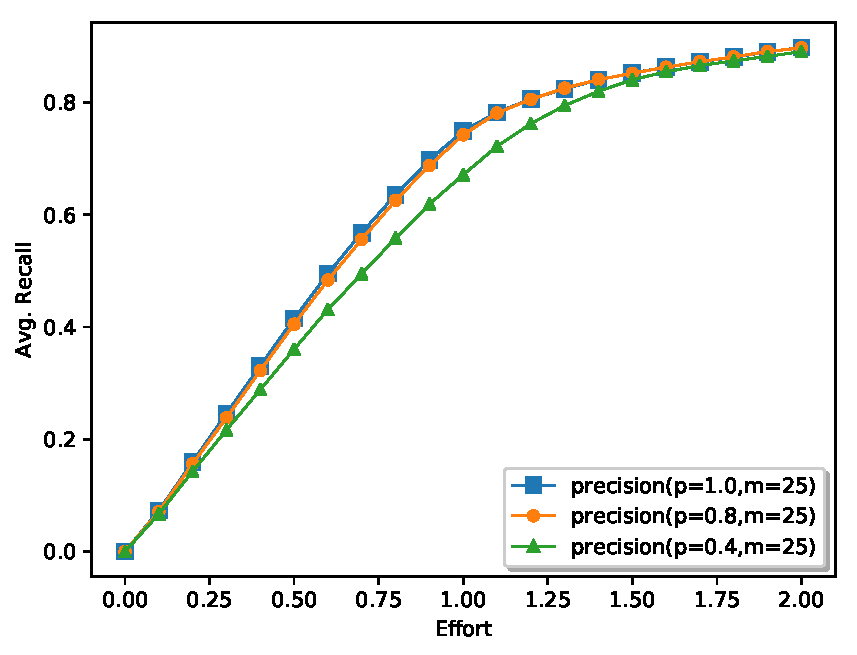
\includegraphics[width=0.7\textwidth]{../plots/precision.pdf}
 \caption{Precision based refreshing vs Static Batch}
\end{figure}
\end{frame}

\begin{frame}{Results}
\begin{figure}
 \centering 
 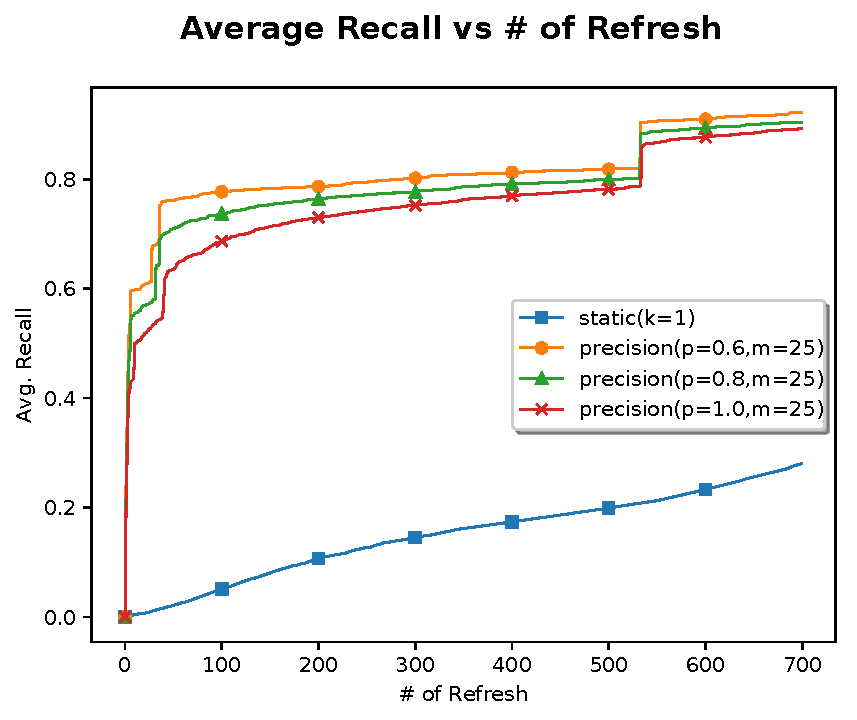
\includegraphics[width=0.7\textwidth]{../plots/prec2.pdf}
 \caption{Precision based refreshing vs Static Batch}
\end{figure}
\end{frame}

\begin{frame}{Results}
\begin{table}[]
\centering
\caption{Recency Weighting}
\label{table.summary}
\resizebox{\textwidth}{!}{%
\begin{tabular}{|c|c|c|c|c|c|}
\hline
\textbf{Strategy} & \begin{tabular}[x]{@{}c@{}}
    \textbf{Avg. Recall}\\ \textbf{@($E_{norm}$=1)}
\end{tabular} & \begin{tabular}[x]{@{}c@{}}
\textbf{Avg. Recall}\\ \textbf{@($E_{norm}$=2)}
\end{tabular} & \begin{tabular}[x]{@{}c@{}}
\textbf{$E_{norm}$ for}\\ \textbf{75\% recall}
\end{tabular}&
\begin{tabular}[x]{@{}c@{}}
    \textbf{Running Time}\\ \textbf{(in min)}
\end{tabular} \\ \hline \hline
\rowcolor{LightCyan}
\texttt{static(k=1)} & 0.750 & 0.926 & 1.021 & 59.59 \\ \hline \hline
\texttt{recency(w=1,it=1000)} &  0.704 & 0.875 & 1.243 & 23.75 \\ \hline
\texttt{recency(w=5,it=1000)} &  0.704 & 0.887 & 1.191 & 26.71 \\ \hline
\texttt{recency(w=10,it=1000)} &  0.707 & 0.891 & 1.206 & 23.30 \\ \hline
\end{tabular}
}
\end{table}
\vskip 0.5cm
\texttt{static(k)}: fixed batch size of \texttt{k}

\texttt{recency(w,it)}: \texttt{it} number of iterations; latest judged document
\texttt{w} times more likely to be sampled than the earliest judged document
\end{frame}


\begin{frame}{Results}
\begin{figure}
 \centering 
 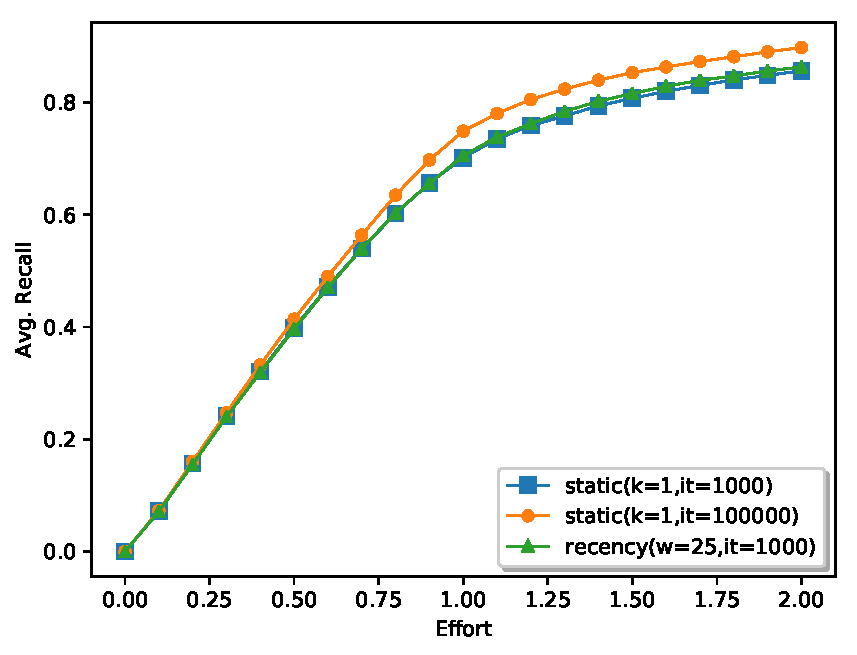
\includegraphics[width=0.7\textwidth]{../plots/recency.pdf}
 \caption{Recency Weighting vs Static Batch}
\end{figure}
\end{frame}



% \section{Implementation}
% \begin{frame}{Implementation}
% \begin{itemize}
%     \item Implementation of BMI in C++
%     \begin{itemize}
%         \item Fast
%         \item Easy to use and configure (CLI/HTTP)
%         \item Extendable (components as abstractions  which can be replaced/modified easily)
%     \end{itemize}
%     \item Useful research tool
%     \item Used in
%     \begin{itemize}
%         \item TREC 2017 Core Track effort by UWatMDS
%         \item User Study and Demo (papers submitted to SIGIR 2018)
%     \end{itemize}
%     \item Operates entirely in-memory
%     \begin{itemize}
%         \item Requires all the documents in the memory (Drawback)
%     \end{itemize}
% \end{itemize}
% \end{frame}


% \subsection{Static Batch Sizes}
% \begin{frame}{Static Batch Sizes}
% Train and score all documents after every $k$ assessments ($k$ is static)
% \vskip 1cm
% $k = 1$
% \begin{itemize}
% \item Effective
% \item High computation cost
% \end{itemize}
% \end{frame}


% \begin{frame}
% \begin{figure}
%  \centering 
%  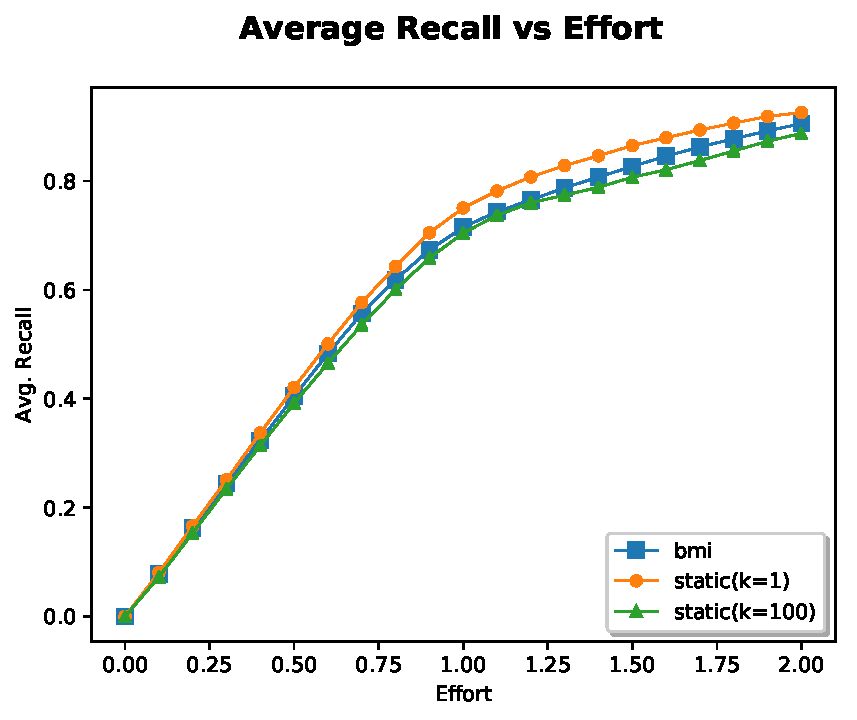
\includegraphics[width=1.0\textwidth]{static1.pdf}
% \end{figure}
% \end{frame}



% \begin{frame}{Partial Refresh}
% This strategy can help with the high memory costs
% \vskip 0.5cm
% Partial Refreshes are fast and performed on small set of data which can be stored in the memory

% \vskip 0.25cm
% Full Refresh can be performed in the background (reading from disk)
% \end{frame}


% \begin{frame}
% \begin{figure}
%  \centering 
%  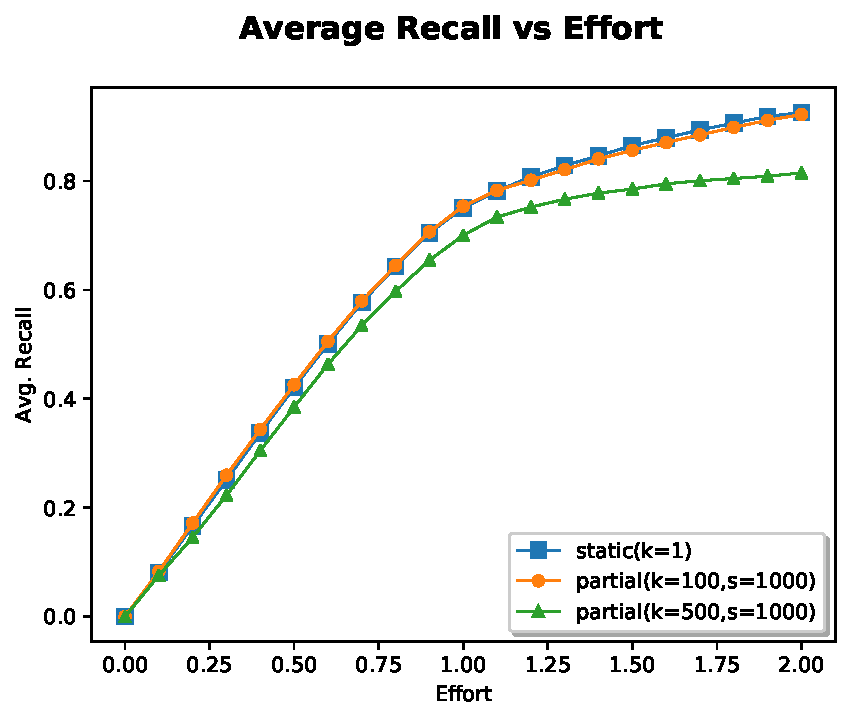
\includegraphics[width=1.0\textwidth]{partial1.pdf}
% \end{figure}
% Parameters
% \begin{itemize}
%     \item Size of partial re-score document set ($s$)
%     \item Period for full refresh ($k$)
% \end{itemize}
% \end{frame}


% \begin{frame}
% \begin{figure}
%  \centering 
%  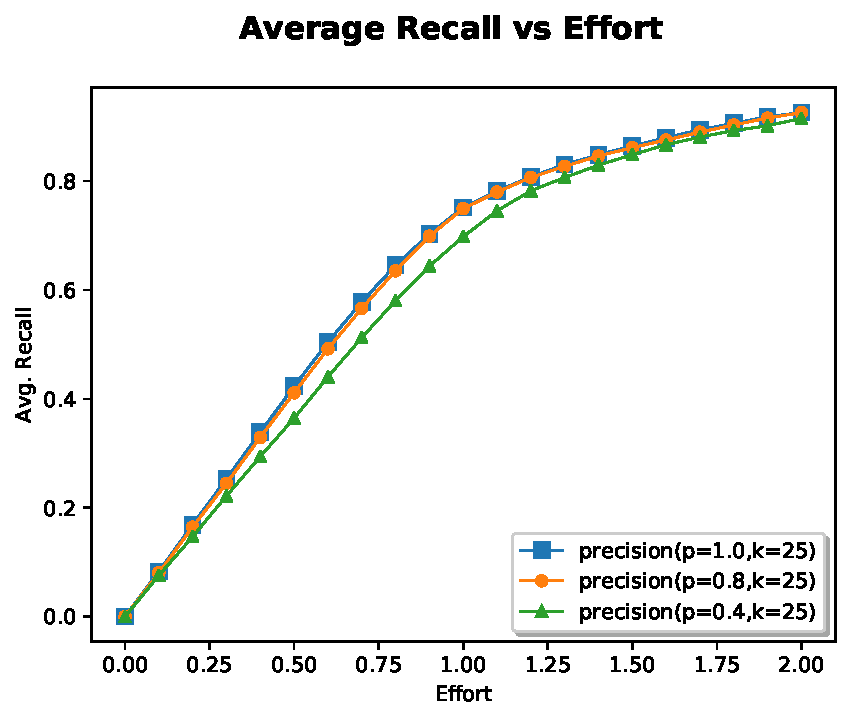
\includegraphics[width=1.0\textwidth]{prec1.pdf}
% \end{figure}
% \end{frame}

% \begin{frame}
% \begin{figure}
%  \centering 
%  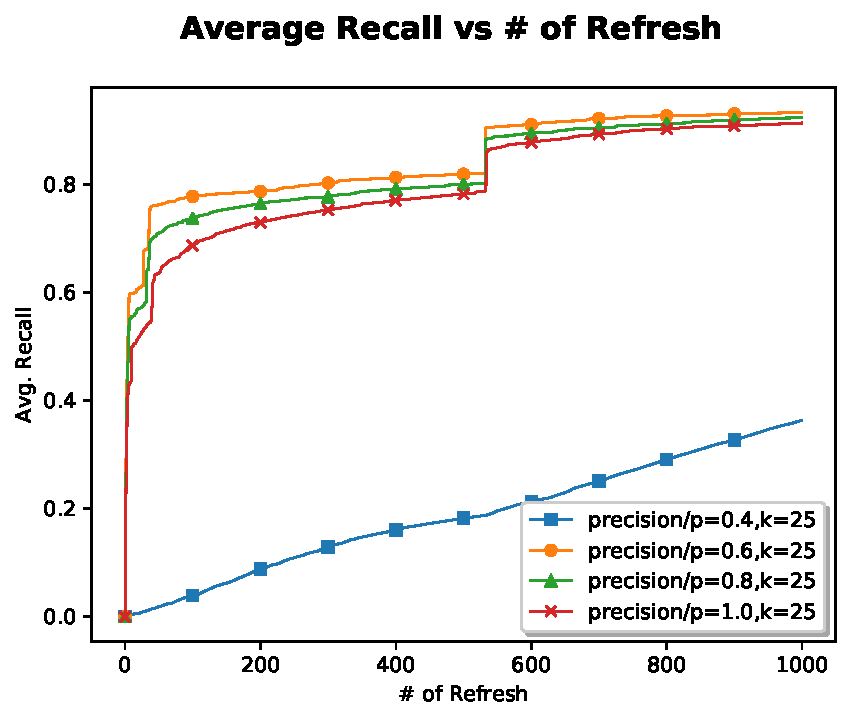
\includegraphics[width=1.0\textwidth]{prec2.pdf}
% \end{figure}
% \end{frame}


% \begin{frame}
% \begin{figure}
%  \centering 
%  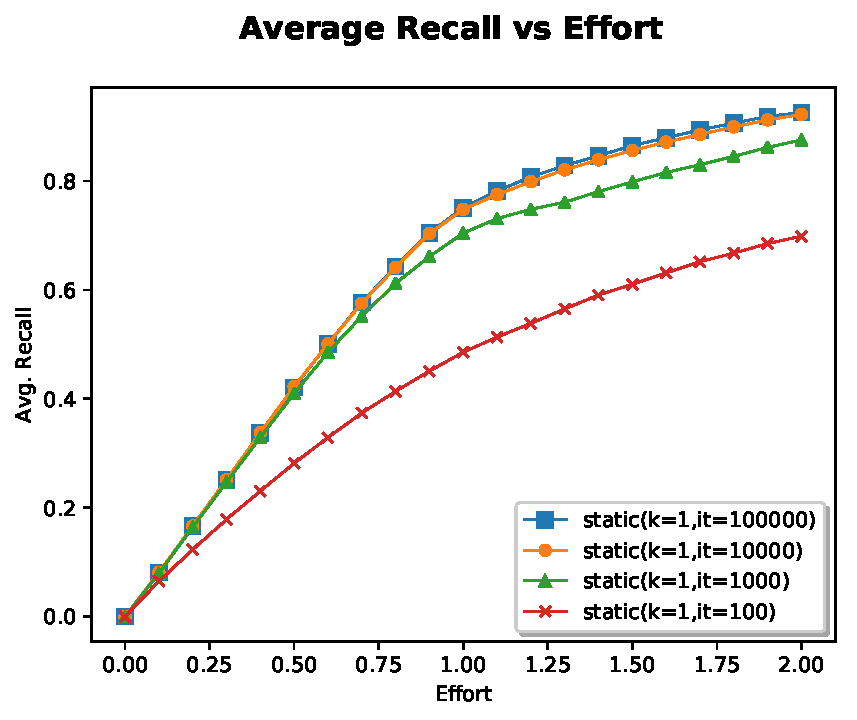
\includegraphics[width=1.0\textwidth]{train1.pdf}
% \end{figure}
% \end{frame}

% \begin{frame}
% \begin{figure}
%  \centering 
%  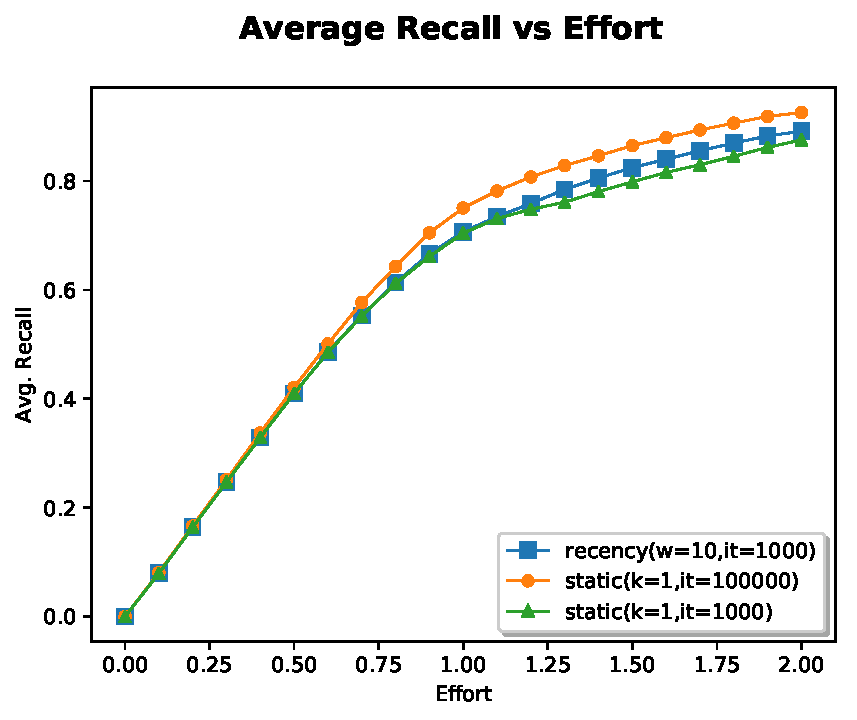
\includegraphics[width=1.0\textwidth]{rec1.pdf}
% \end{figure}
% \end{frame}

\begin{frame}{Static Batches and Responsiveness}
    \texttt{static(k=1)} is consistently outperforms other strategies in term of
    effectiveness

    \vskip 0.5cm
    Even if a refresh is performed within 1 second, frequent pauses harm user
    experience and productivity
\end{frame}

\begin{frame}{Static Batches and Responsiveness}
    Asynchronous refreshes
    \begin{itemize}
        \item Used by UWaterlooMDS in TREC 2017 Core
            Track~\cite{zhang2017uwaterloomds}
        \item Immediately show the user documents from the old review queue
        \item Refresh in background and replace the review queue when done
            \pause
        \item Delays the effect of user feedback on review queue by
            $\lceil \frac{t_r}{t_u} \rceil$ judgments
            \begin{itemize}
                \item $t_r$ = time to perform one refresh (avg. 1.71s)
                \item $t_u$ = time assessor takes to review a document (avg. 13s)
            \end{itemize}
    \end{itemize}
\end{frame}

\begin{frame}{Static Batches and Responsiveness}
    If two refreshes can be performed while the assessor is reading a document
    ($2t_r \le t_u):

    \vskip 0.5cm
    Perform two refreshes in background; one for each possible future judgment
\end{frame}


\section{Conclusion}
\begin{frame}{Summary}
\begin{itemize}
    \item Frequent refreshing helps achieving higher recall using lesser
       assessment effort
       \vskip 0.5cm
    \item Static batch size of 1 performs great but is computationally expensive
        \begin{itemize}
            \item Practical for reasonably sized datasets and modern hardware
            \item Various alternative strategies (partial and precision based
                refreshing) can achieve similar effectiveness with reduced
                computations
        \end{itemize}
    \item Recency weighting doesn't help effectiveness
    \item A modern implementation of CAL
\end{itemize}
\end{frame}

\begin{frame}{Future Work}
\begin{itemize}
    \item Optimize of memory efficiency
        \begin{itemize}
            \item Large datasets like ClueWeb, Twitter, and so on.
        \end{itemize}
    \item Vast literature dealing with scaling/optimizing various steps in CAL
        \begin{itemize}
            \item Online training
            \item Large scale classification
        \end{itemize}
\end{itemize}
\end{frame}
\begin{frame}{Bibliography}
\fontsize{6}{7.2}\selectfont
\bibliographystyle{unsrt}
\bibliography{talk}
\end{frame}
\end{document}

